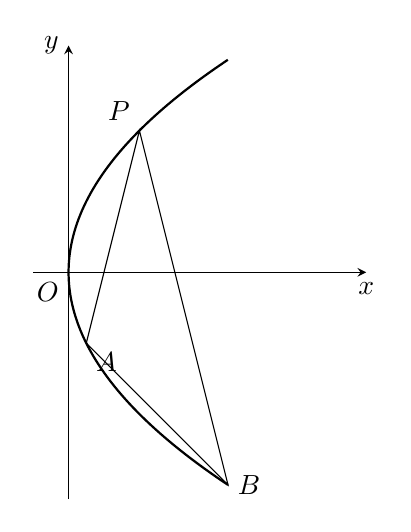
\begin{tikzpicture}[>=stealth, scale=0.9]
  % 坐标轴
  \draw[->] (-0.5, 0) -- (4.2, 0) node[below] {$x$};
  \draw[->] (0, -3.2) -- (0, 3.2) node[left] {$y$};
  \node[below left] at (0, 0) {$O$};

  % 抛物线 y^2 = 4x (x = y^2 / 4)
  \draw[thick, domain=-3.0:3.0, samples=100] plot ({0.25*\x*\x}, {\x});

  % 关键点坐标 (x = y^2/4)
  % P(1, 2)
  \coordinate (P) at (1.0, 2.0);
  % A(0.25, -1.0)
  \coordinate (A) at (0.25, -1.0);
  % B(2.25, -3.0)
  \coordinate (B) at (2.25, -3.0);

  % 连线构成三角形 PAB
  \draw[thin] (P) -- (A) -- (B) -- cycle;

  % 点标注
  \node[above left] at (P) {$P$};
  \node[below right] at (A) {$A$};
  \node[right] at (B) {$B$};
\end{tikzpicture}
